\documentclass[a4paper,11pt]{article}

\usepackage[utf8]{inputenc}
\usepackage[T1]{fontenc}
\usepackage{babel}
\usepackage[top=2.5cm, bottom=2.5cm, left=2.5cm, right=2.5cm]{geometry}
\usepackage{xcolor}
\usepackage{hyperref}
\usepackage{titlesec}
\usepackage{enumitem}
\usepackage{mdframed}
\usepackage{fancyhdr}
\usepackage{graphicx}

% Couleurs
\definecolor{violetuniv}{RGB}{100, 50, 150}
\definecolor{rougetitre}{RGB}{200, 50, 50}
\definecolor{borduregrise}{RGB}{180, 180, 180}
\definecolor{rose}{RGB}{180, 50, 100}

% Liens hypertexte
\hypersetup{
    colorlinks=true,
    linkcolor=violetuniv,
    urlcolor=violetuniv,
}

% Style des titres de section
\titleformat{\section}{\large\bfseries}{}{0em}{}
\titleformat{\subsection}{\normalsize\bfseries}{}{0em}{}
\titleformat{\subsubsection}{\normalsize\bfseries}{}{0em}{}

% En-tête
\pagestyle{fancy}
\fancyhf{}
\renewcommand{\headrulewidth}{0.4pt}
\fancyhead[L]{\small\textcolor{violetuniv}{Conception Web -- Semestre 2}}
\fancyfoot[C]{\thepage}

% Environnement "À faire"
\newmdenv[
    linecolor=borduregrise,
    backgroundcolor=white,
    linewidth=1pt,
    leftmargin=0pt,
    rightmargin=0pt,
    innerleftmargin=10pt,
    innerrightmargin=10pt,
    innertopmargin=8pt,
    innerbottommargin=8pt,
]{afaire}

\begin{document}

% ============================================================
% PAGE DE PRÉSENTATION
% ============================================================
\thispagestyle{empty}
\vspace*{3cm}

\begin{center}
    {\small\textcolor{violetuniv}{Université d'Avignon -- CERI}}\\[0.5cm]
    {\small\textcolor{violetuniv}{Licence Informatique -- Semestre 2}}\\[2cm]

    {\rule{\linewidth}{0.5pt}}\\[0.4cm]
    {\LARGE\bfseries Conception Web}\\[0.3cm]
    {\large TP2 -- CSS}\\[0.4cm]
    {\rule{\linewidth}{0.5pt}}\\[2cm]

    {\large Module : S-E06-0158}\\[0.5cm]
    {\large Année universitaire 2025--2026}\\[3cm]

    \begin{tabular}{ll}
        \textbf{Enseignant :} & Fabrice Lefèvre \\
        \textbf{Niveau :}     & Licence 1 Informatique \\
        \textbf{Semestre :}   & Semestre 2 \\
    \end{tabular}
\end{center}

\vfill

\begin{center}
    \textcolor{borduregrise}{\rule{\linewidth}{0.3pt}}\\[0.3cm]
    {\small\textit{Ce document présente le sujet du TP CSS du module Conception Web.}}
\end{center}

% ============================================================
\newpage
\fancyhead[R]{\small TP -- CSS}

{\Large\bfseries TP -- CSS}

\bigskip

\section{CSS}

Avant de passer à l'utilisation de frameworks CSS, comme W3.CSS, il convient de s'assurer d'un peu plus de maîtrise du CSS \textit{\textbf{de base}}.

\section{Attribut \texttt{style}, feuilles de style interne et externe}

Le nom \textcolor{rose}{\texttt{Cascading}} (le ``C'' dans CSS) vient de la possibilité offerte par CSS de définir les propriétés de style à plusieurs niveaux dans les documents HTML. Les trois niveaux possibles sont :

\begin{enumerate}
    \item la balise avec l'attribut \textcolor{rose}{\texttt{style}} : les propriétés sont données directement au niveau de la balise concernée (e.g. \textcolor{rose}{\texttt{<p style='color:red'>Contenu ...</p>}}).\\
    \textcolor{rougetitre}{\textbf{Attention}} : on peut donner une \textbf{liste} de propriétés (séparées par des ``\texttt{;}") ;
    \item une feuille de style interne : les propriétés sont regroupées dans l'entête (\texttt{<head>}) du document HTML (e.g. \textcolor{rose}{\texttt{<head><style type='text/css'> body\{background-color:\#8c9be7\}</style></head>}}) ;
    \item une feuille de style externe : les propriétés sont regroupées dans un document CSS séparé, lié aux documents HTML à l'aide de la balise \textcolor{rose}{\texttt{<link>}}.
\end{enumerate}

\textcolor{rougetitre}{\textbf{Conseil :}} Par la suite, dans la mesure où on ne modifie souvent qu'un seul document HTML dans nos TP, on pourra se contenter d'utiliser une feuille de style interne. Mais la feuille de style externe est fortement conseillée lorsque l'on conçoit un site complet : un document CSS est alors partagé par tous les documents HTML du site et les modifications éventuelles sont simplifiées. De plus vous aurez rapidement recours à des librairies CSS déjà écrites et donc fournies en ligne.

% ============================================================
\section{A. Utilisation des identifiants et des classes}

\begin{afaire}
\textbf{A faire :}

Téléchargez l'archive du TP, après ce sujet.
\end{afaire}

\subsection{1. Utilisation d'identifiants}

\begin{afaire}
\textbf{A faire :}

\begin{enumerate}
    \item Donner un identifiant unique à chacun des éléments \textcolor{rose}{\texttt{div}} de la page HTML, ainsi qu'à l'élément \textcolor{rose}{\texttt{cite}} final.
    \item Ajouter le code CSS à l'entête de votre fichier pour que le texte du deuxième \textcolor{rose}{\texttt{div}} soit de couleur orange et de taille \texttt{small}. Toutes les demandes suivantes devront venir compléter les déclarations CSS du header.
\end{enumerate}
\end{afaire}

\subsection{2. Utilisation de classes}

\begin{afaire}
\textbf{A faire :}

\begin{enumerate}
    \item Appliquez les classes suivantes aux colonnes du tableau (après le texte ``Paragraphe 12'') :
    \begin{itemize}
        \item la classe \textcolor{rose}{\texttt{produit}} à la première colonne
        \item la classe \textcolor{rose}{\texttt{reference}} à la deuxième colonne
        \item la classe \textcolor{rose}{\texttt{general}} aux autres colonnes
    \end{itemize}
\end{enumerate}

\textcolor{rougetitre}{\textbf{Conseil :}}
\begin{enumerate}
    \item contrairement aux lignes du tableau (\texttt{<tr>}), les colonnes sont définies implicitement en HTML. Mais il est possible de les définir explicitement lorsqu'on veut leur associer des propriétés particulières. Il suffit de trouver la bonne balise ?
    \item Puis définir les mises en forme associées à chaque classe : colorier le fond de la colonne
    \begin{itemize}
        \item \ldots en jaune pour la classe \textcolor{rose}{\texttt{produit}}
        \item \ldots en orange pour la classe \textcolor{rose}{\texttt{reference}}
        \item \ldots en rouge pour la classe \textcolor{rose}{\texttt{general}}
    \end{itemize}
\end{enumerate}
\end{afaire}

% ============================================================
\section{B. Sélecteurs contextuels (ou ``combinatoires'')}

\subsection{1. Sélecteur contextuel ``simple''}

\begin{afaire}
\textbf{A faire :}

Tous les titres de niveau 3 du premier \textcolor{rose}{\texttt{div}} doivent être de couleur marron et être centrés.
\end{afaire}

\subsection{2. Sélecteur contextuel et pseudo-élément}

\begin{afaire}
\textbf{A faire :}

La première lettre (\textcolor{rose}{\texttt{first-letter}}) de chaque élément \texttt{p} d'un \textcolor{rose}{\texttt{blockquote}} du premier \textcolor{rose}{\texttt{div}} doit être de couleur rouge et de graisse\ldots{} grasse (\textcolor{rose}{\texttt{bold}}).
\end{afaire}

% ============================================================
\section{C. Formatage de la police}

\begin{afaire}
\textbf{A faire :}

Appliquer les styles suivants :
\begin{enumerate}
    \item L'ensemble du document doit être de police (dans cet ordre de préférence) : Papyrus, Lucida Console ou défaut (proposer une famille de police générique par défaut).
    \item Les titres doivent être d'une police différente du reste du document, à choisir.
    \item La première lettre de chaque élément \textcolor{rose}{\texttt{blockquote}} du premier \textcolor{rose}{\texttt{div}} doit être de police Helvetica et de taille deux fois et demie la taille par défaut (c'est-à-dire à 250\% !).
    \item Chaque cellule-titre du tableau doit être en petites majuscules (\textcolor{rose}{\texttt{small-caps}}).
\end{enumerate}
\end{afaire}

% ============================================================
\section{D. Formatage du texte}

\begin{afaire}
\textbf{A faire :}

Appliquer les styles suivants :
\begin{enumerate}
    \item Chaque élément \textcolor{rose}{\texttt{blockquote}} doit être indenté de 6em.
    \item Pour chaque titre de niveau 2 du premier \texttt{div}, la direction du texte doit être changé de droite à gauche (ex: titre devient ertit), mais garder l'alignement à gauche.
    \item Le texte de chaque cellule de titre du tableau doit être surligné (\textcolor{rose}{\texttt{overline}}) avec un style en vague (\textcolor{rose}{\texttt{wavy}}).
\end{enumerate}
\end{afaire}

% ============================================================
\section{E. Couleurs et fonds}

\begin{afaire}
\textbf{A faire :}

\begin{enumerate}
    \item En utilisant l'image fournie dans l'archive téléchargée (lien direct : \textcolor{violetuniv}{petit chien rigolo}).
    \item Appliquer les styles suivants :
    \begin{enumerate}
        \item Le fond de l'ensemble du document doit être de couleur bleu clair.
        \item Le fond du dernier élément \textcolor{rose}{\texttt{div}} doit être bleu plus clair.
        \item Placer l'image du petit chien en fond (\textcolor{rose}{\texttt{background}}) du premier \textcolor{rose}{\texttt{div}}, la positionner en bas à gauche et la répéter horizontalement.
    \end{enumerate}
\end{enumerate}
\end{afaire}

% ============================================================
\section{F. Boîtes/blocs}

\subsection{1. Bordures}

\begin{afaire}
\textbf{A faire :}

\begin{enumerate}
    \item Ajouter une bordure large de couleur bleu et en saillie (\textcolor{rose}{\texttt{groove}}) au paragraphe intitulé ``Border''.
    \item Ajouter aussi un \textcolor{rose}{\texttt{padding}} de \texttt{20ex}.
\end{enumerate}
\end{afaire}

\subsection{2. Flottement de bloc}

\begin{afaire}
\textbf{A faire :}

\begin{enumerate}
    \item Faire flotter (\textcolor{rose}{\texttt{float}}) le ``petit texte à droite'' à \ldots droite.
    \item Ensuite vous pouvez tester le comportement vis-à-vis de la propriété d'alignement du texte (en observant les variations selon le changement de valeur).
\end{enumerate}
\end{afaire}

% ============================================================
\section{G. Listes}

\begin{afaire}
\textbf{A faire :}

\begin{enumerate}
    \item Modifier le style des listes :
    \begin{itemize}
        \item Les listes non ordonnées doivent être repérées par des puces disques (\textcolor{rose}{\texttt{disc}})
        \item Les listes ordonnées imbriquées au deuxième niveau (\textcolor{rose}{\texttt{ol ol}}) doivent avoir des puces numériques en japonais (\textcolor{rose}{\texttt{hiragana}})
    \end{itemize}
    \item Tester l'effet de cette modification sur une liste \textbf{qui vous devrez ajouter} après la seconde partie du document.
\end{enumerate}
\end{afaire}

% ============================================================
\section{H. Positionnement}

Une fois les principes de bases acquis, découvrir CSS se résume à parcourir les documentations à la recherche des (bonnes) propriétés qui peuvent être modifiées. Il est difficile de se faire une idée a priori des réalisations graphiques que l'on peut obtenir avec une bonne utilisation des CSS. Pour cela, une fois de plus, la méthode la plus sûre est l'exemple !

A ce titre le site \textcolor{violetuniv}{CSS Zen Garden} est une bonne source d'inspiration puisqu'il met en oeuvre concrètement le principe de séparation du fond et de la forme : le fond du document est un fichier html et la forme est gérée exclusivement dans un fichier CSS externe. Ainsi, en changeant le fichier CSS, on modifie la présentation sans JAMAIS retoucher au document html. Pour les autres sites en général, il est intéressant de se rappeler que les fichiers externes CSS utilisés par les documents html sont TOUJOURS accessibles en ligne : il suffit de récupérer leur URL (dans le \textcolor{rose}{\texttt{<link...>}} du fichier html) et de la saisir dans la barre d'adresse.

\textbf{Attention} : cet exercice n'est pas à réaliser avec le framework W3.CSS.

\begin{afaire}
\textbf{A faire :}

\begin{enumerate}
    \item Reproduisez l'exemple ci-dessous en utilisant les propriétés de positionnement absolu et la notion de \texttt{z-index}
    (voir annexe \ref{annexe:position1}, page \pageref{annexe:position1}).
    \item En récupérant les images \texttt{papillon.gif} et \texttt{papillon2.gif}, reproduisez l'exemple suivant
    (voir annexe \ref{annexe:position2}, page \pageref{annexe:position2}).
\end{enumerate}
\end{afaire}

\vspace{1em}
\noindent\textcopyright{} Fabrice Lefèvre, 2026.

\vspace{0.5em}
\noindent\textit{Last modified: Saturday, 28 March 2026, 7:48 PM}

% ============================================================
% ANNEXES
% ============================================================
\newpage
\fancyhead[R]{\small Annexes}
\appendix

\section{Exemple de positionnement 1 -- TP CSS}
\label{annexe:position1}

Reproduire ce résultat en utilisant le positionnement absolu et \texttt{z-index}.

\bigskip

\begin{center}
    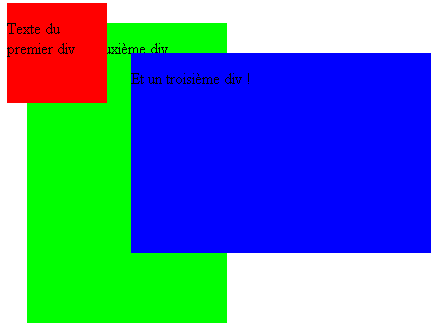
\includegraphics[width=0.55\textwidth]{position1.png}
\end{center}

\section{Exemple de positionnement 2 -- TP CSS}
\label{annexe:position2}

Reproduire ce résultat en ajoutant les images \texttt{position1.png} et \texttt{position2.png}.

\bigskip

\begin{center}
    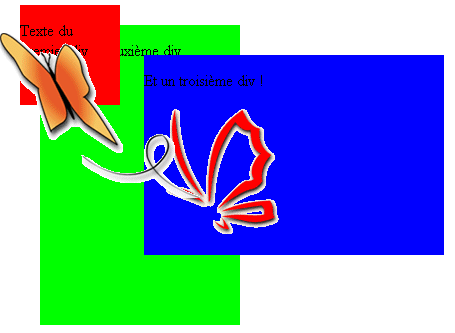
\includegraphics[width=0.55\textwidth]{position2.png}
\end{center}

\end{document}